\section{Methodology}
The project will consist of 4 main steps:
\begin{enumerate}
    \item Data Collection and loading
    \item Data Preprocessing
    \item Lung segmentation
    \item GGO visualization and Evaluation
\end{enumerate}

The overall methodology is illustrated in figure \ref{fig:methodology}:
\begin{figure}[h]
    \centering
    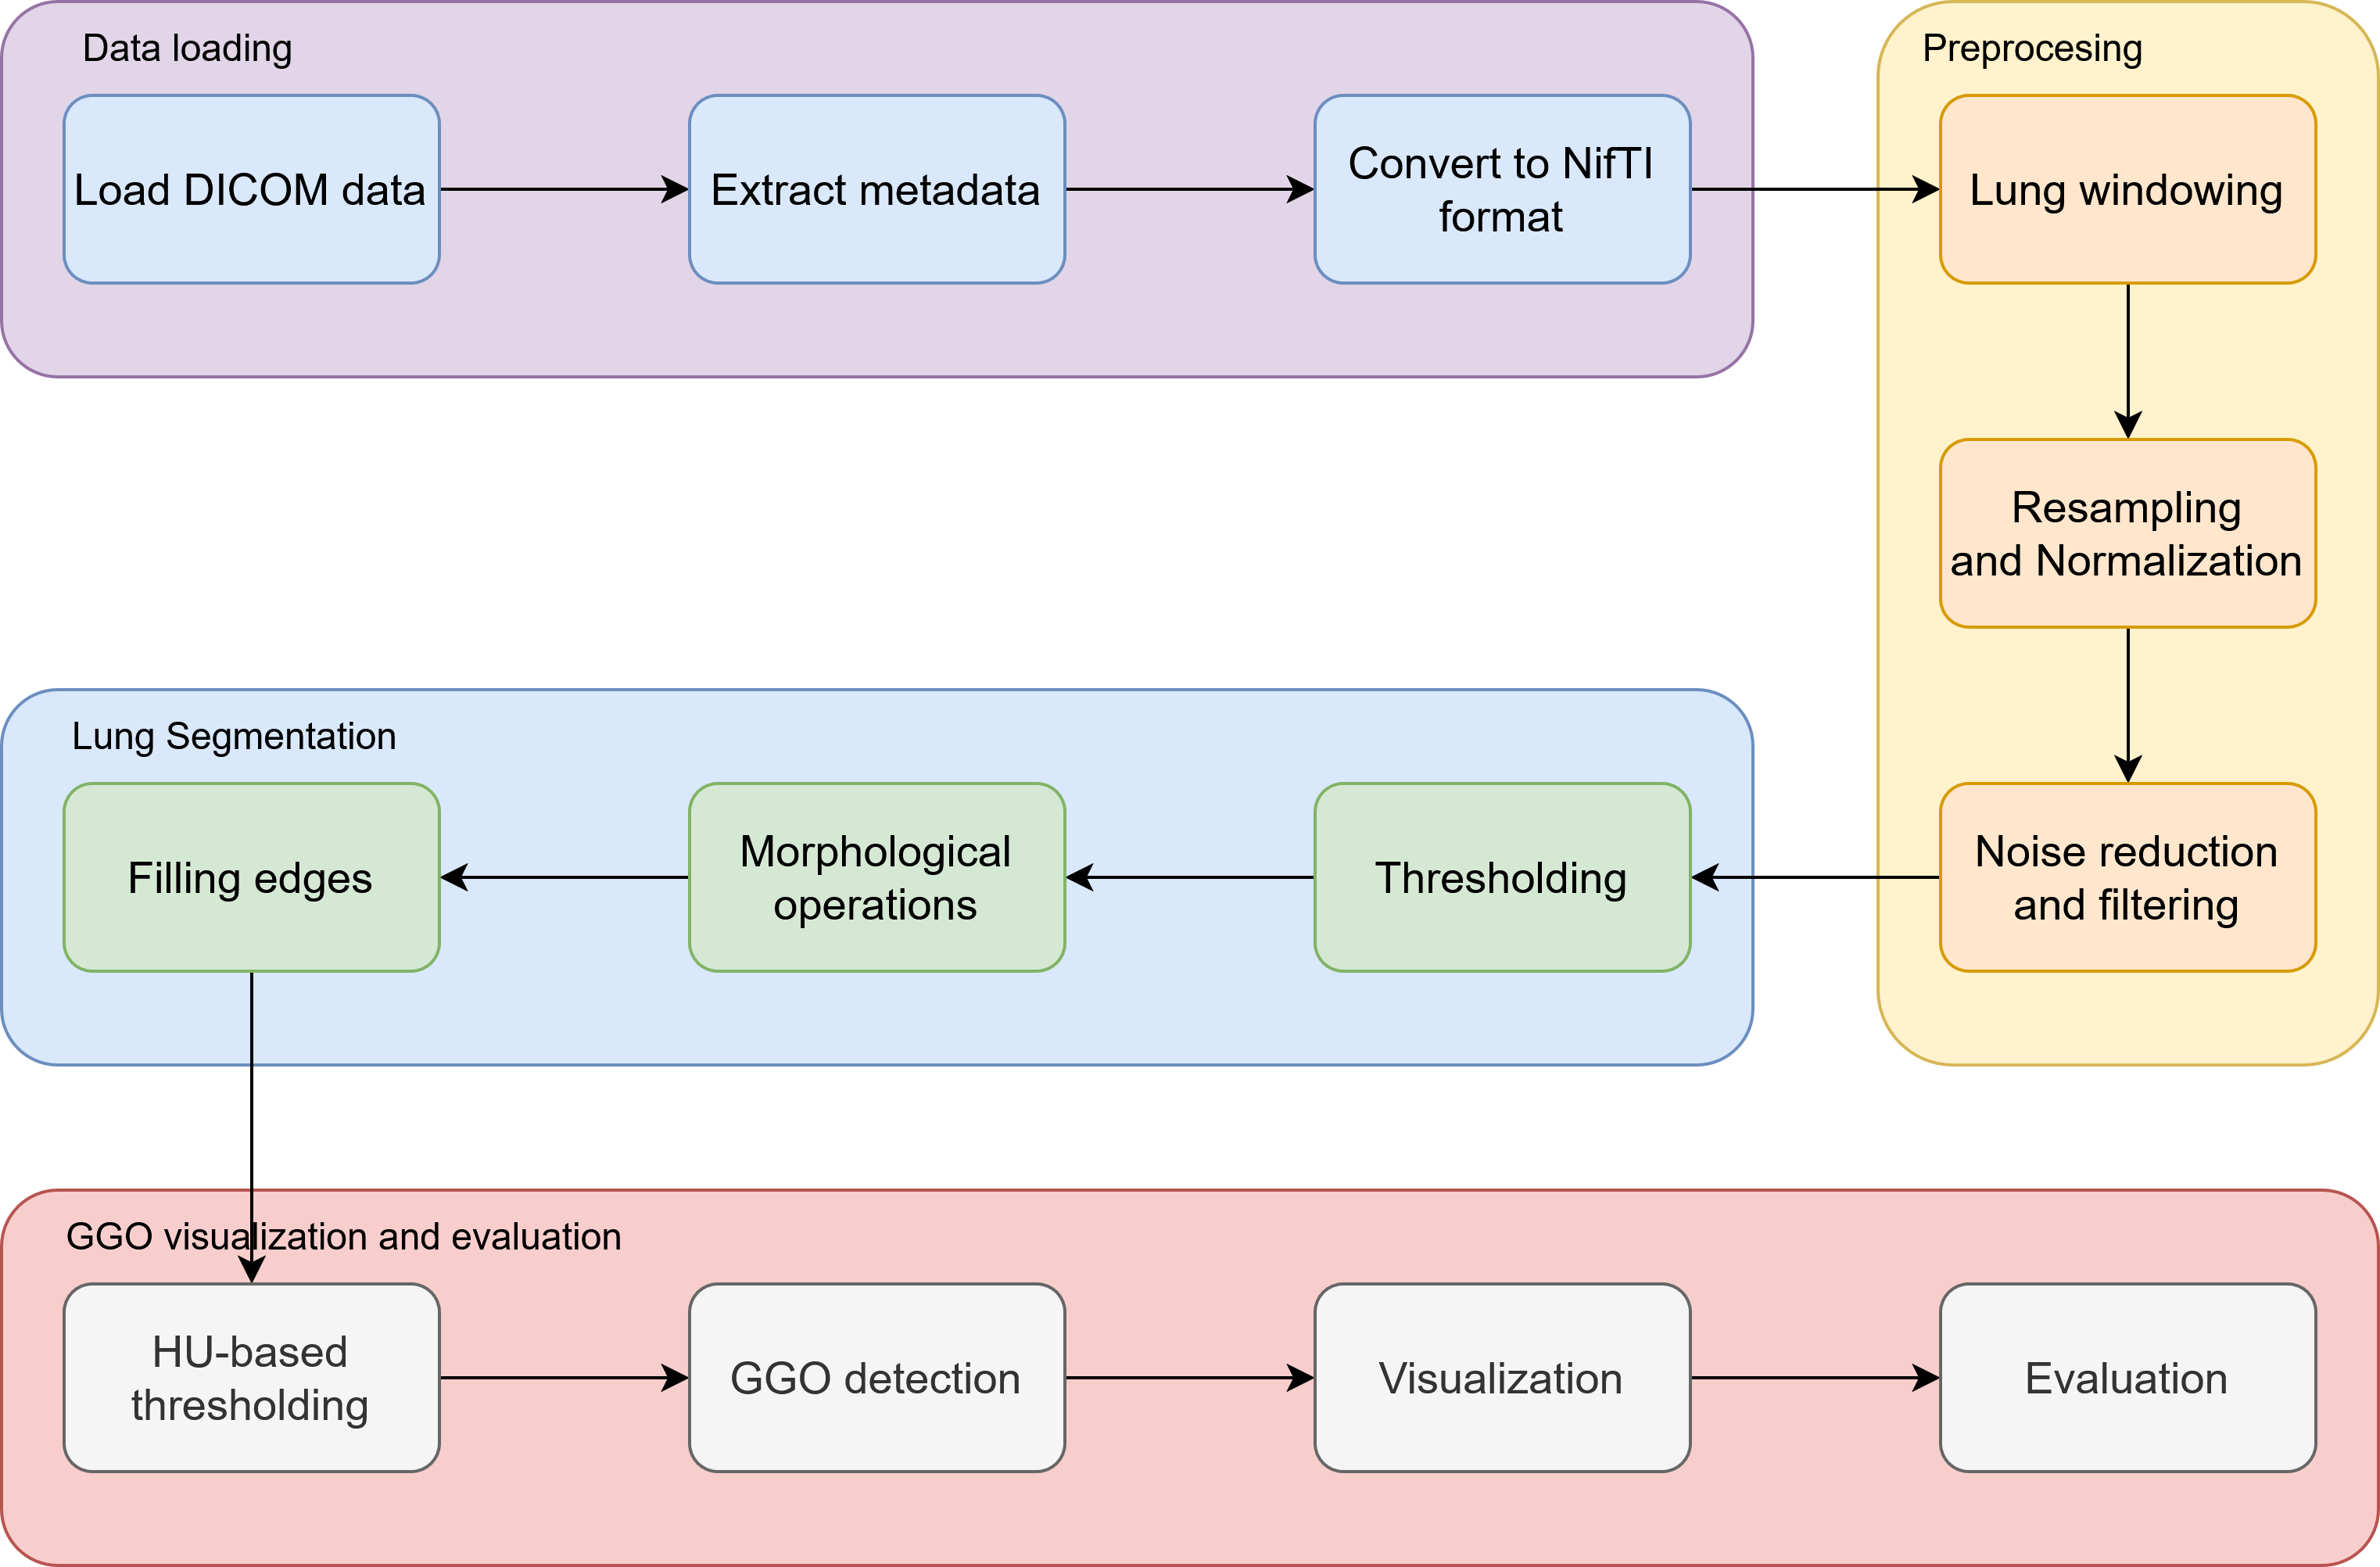
\includegraphics[width=0.8\textwidth]{methodology.png}
    \caption{Methodology Overview}
    \label{fig:methodology}
\end{figure}

\subsection{Data Collection and loading}
We will use the publically available LIDC-IDRI dataset \cite{armato2011lung} which contains lung CT scans from the Lung Image
Database Consortium (LIDC) and Image Database Resource Initiative (IDRI).
The dataset contains over 11000 clinical thoracic CT scans in DICOM format. The Python library "pylidc" is the standard tool used
to query and visualize this data. The data will be loaded using Python libraries such as "pydicom".

Once the dataset is loaded, we will extract their metadata. The metadata is primarily contained within the DICOM headers of the
images and the XML files that hold the radiologist's findings. The LIDC-IDRI dataset provides metadata under three categories:
\begin{itemize}
    \item \textbf{Scan and Patient information: }Includes slice thickness, pixel spacing, intravenous contrast usage
    \item \textbf{Annotations: }Includes type of Lesion and ROI maps
    \item \textbf{Nodule characteristics: }For nodules > 3mm, the metadata includes subjective ratings from 1 to 5 for nine specific features
\end{itemize}

Once the metadata is extracted, we will convert the DICOM images to standard NifTI format using the "dcm2niix" tool for easier
processing in later stages. This conversion helps for compatibility with various medical image processing libraries as DICOM is
complex and bulky for analysis.

\subsection{Data preprocessing}
After loading and extracting metadata, the data will be preprocessed to improve the overall quality of the CT images before segmentation.
This step includes:
\begin{itemize}
    \item Windowing the images to focus on lung tissue
    \item Resampling and Normalizing pixel intensities
    \item Removing noise and artifacts
\end{itemize}

We will apply a lung-specific window level and width to enhance the visibility of lung tissues. This is a medical image convention
used to clip the Housenfield range is by choosing a central intensity. Next, resampling will be
done to ensure uniform voxel spacing across all scans, which is important for accurate segmentation. This is done because, different scanners
may produce images with varying resolutions. Resampling changes the resolution to a standard size such as 1mm x 1mm x 1mm.
We will use interpolation methods such as linear or cubic interpolation for this purpose.

Once resampling is done, normalization of pixel intensities will be performed to standardize the intensity values across different
scans. This makes mathematical operations more stable and removes dependency on absolute HU values for algorithms.
Noise reduction techniques such as Gaussian, Median or Bilateral filtering will be applied to reduce random variations in pixel intensities
while preserving important structures like GGO boundaries. Since CT images inherently contain quantum noise, it can create false GGO detections.

\subsection{Lung Segmentation}
In order to perform Lung segmentation, we will use a combination of intensity based thresholding and morphological image processing techniques.
First we will find the real area of the lung in $mm^2$ by finding the real size of the pixel dimensions. Nex, we will binarize the
images using intensity thresholding to separate lung tissues from the background. We expect lungs to be in the Housendfield unit
range of [-1000,-300]. To this end, we need to clip the image range to [-1000,-300] and binarize the values to 0 and 1.

Then we need to find the contours of the lung areas. In computer vision, a contour is a set of points that describe a line or area.
So for each detected contour we will not get a full binary mask but rather a set with a multiple x and y values.
In order to isolate the desired area we will use the marching squares algorithm[]. Using the possible contours, we will extract the
lungs using 2 constraints:
\begin{itemize}
    \item The contour of the lungs must be a closed set
    \item The contour must have a minimum volume of 2000 pixels to represent the lungs
\end{itemize}

Using these 2 assumptions, we will convert the contours into a binary mask representing the lung areas by using the "pillow"
Python library to draw a polygon connecting the contours
After obtaining the binary mask of the lungs, we will save it as a NifTI file and use it for further processing.
Finally, we will do element-wise multiplication between the CT image and the lung mask we obtained to get only the lungs.

\subsection{GGO Visualization and Evaluation}
After segmenting the lungs, we will focus on visualizing the GGO regions within the lung areas. We will assume that if there is a
pixel with an intensity value between -500 HU and -700 HU inside the lung area then we will consider it as a GGO area.
However, this threshold range may also include vessels within the lung parenchyma.
To address this issue, we will apply vessel removal techniques to reduce false positive detections. Since vessels appear
as elongated, tubular structures, we will use morphological opening operations using a circular structuring element to remove them.
Then, we will set the zeros that resulted from the previous element-wise multiplication to -1000 and finally keep only the
intensities that are between -500 and -700 as GGO areas.

Once the GGO area has been identified, we will visualize it by overlaying the detected GGO regions on the original CT images using
pseudo-coloring techniques. We will also visualize the original image alongside the segmented GGO area side-by-side using a User Interface.
Finally, we will evaluate the effectiveness of the GGO segmentation using manually annotated contours provided in the XML files of the LIDC-IDRI dataset.
\hyperref[contents]{\small Back to Table of Contents}